\documentclass{standalone}
\usepackage{tikz}

%Inicio del preambulo

\tikzstyle{startstop} = [rectangle, rounded corners, minimum width=3cm, minimum height=1cm,text centered, draw=black, fill=red!50!blue!40]
\tikzstyle{arrow} = [thick,->,>=stealth]

%Fin del preambulo

\begin{document}
    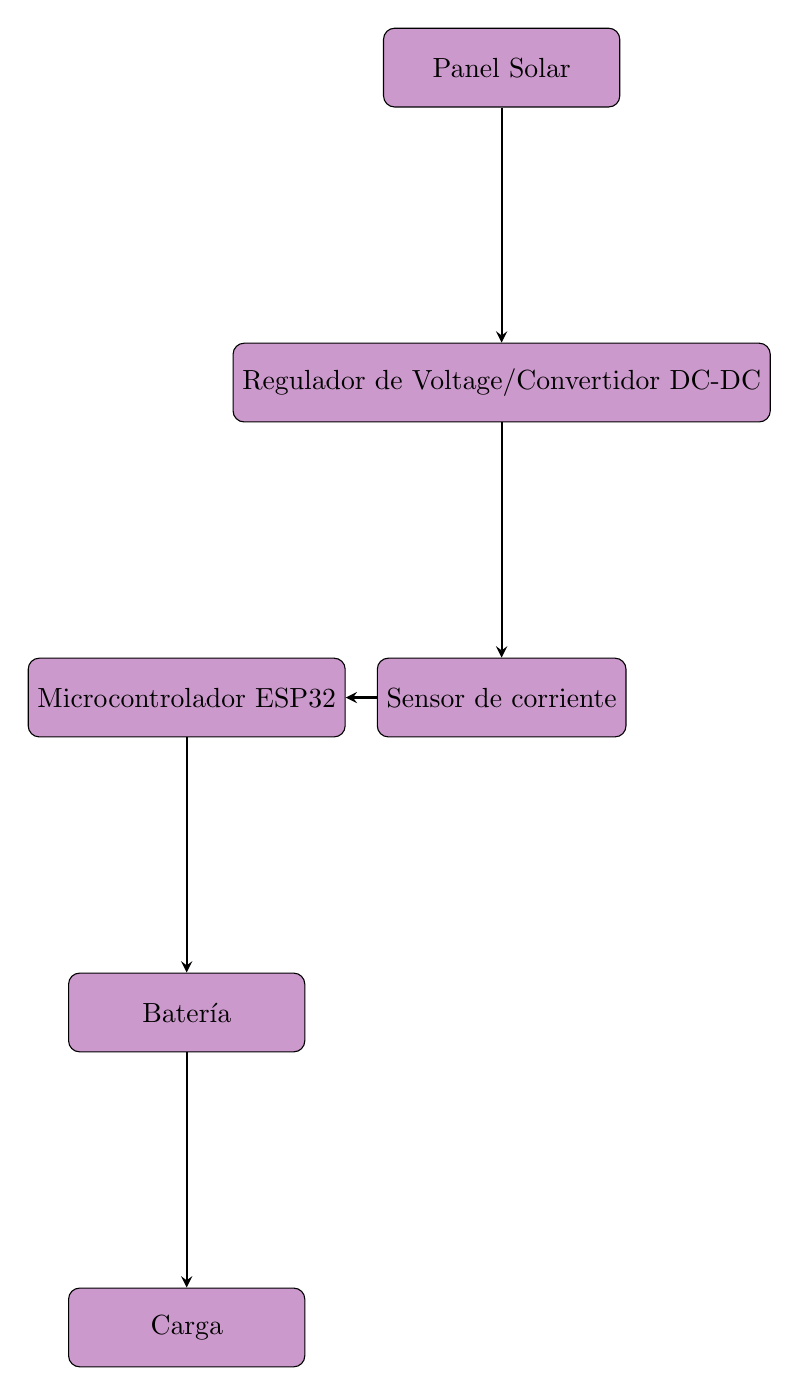
\begin{tikzpicture}[node distance=4cm]
      \node (Solarcell) [startstop] {Panel Solar};
      \node (Regulator) [startstop, below of = Solarcell] {Regulador de Voltage/Convertidor DC-DC};
      \node (CurrentSensor) [startstop,below of = Regulator] {Sensor de corriente};
      \node (Micro) [startstop,left of = CurrentSensor] {Microcontrolador ESP32};
      \node (Battery) [startstop,below of = Micro] {Batería};
      \node (Load) [startstop,below of = Battery] {Carga};
      
      \draw[arrow] (Solarcell) -- (Regulator);
      \draw[arrow] (Regulator) -- (CurrentSensor);
      \draw[arrow] (CurrentSensor) -- (Micro);
      \draw[arrow] (Micro) -- (Battery);
      \draw[arrow] (Battery) -- (Load);
    \end{tikzpicture}
\end{document}